\section{Einführung}

\subsection{Klassifizierung}\script{7}\\
\begin{tabular}{C{4.5cm}|C{4.5cm}}
	\textbf{Energiesignal:} $E = \int_{-\infty}^{\infty}|x(t)|^2dt < \infty$
	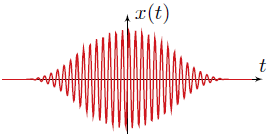
\includegraphics[width=0.4\columnwidth]{Images/energiesignal}
	& \textbf{Leistungssignal:} $P =\lim\limits_{T\rightarrow\infty}\frac{1}{T}\int_{-T/2}^{T/2}|x(t)|^2dt < \infty$
	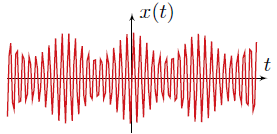
\includegraphics[width=0.4\columnwidth]{Images/leistungssignal} \\ \midrule
	\textbf{Aperiodisch:} $x(t) \neq x(t + nT)$
	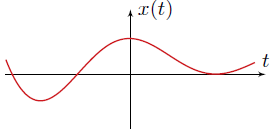
\includegraphics[width=0.4\columnwidth]{Images/apreiodisch}
	& \textbf{Periodisch:} $x(t) = x(t + nT)$
	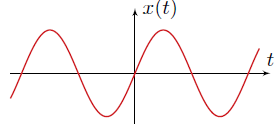
\includegraphics[width=0.4\columnwidth]{Images/periodisch} \\ \midrule
	\textbf{Deterministisch:} $x(t) = f(t)$ Verlauf vorbestimmt
	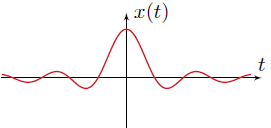
\includegraphics[width=0.4\columnwidth]{Images/deterministisch}
	& \textbf{Stochastisch:} $x(t) = ???$ Verlauf Zufällig
	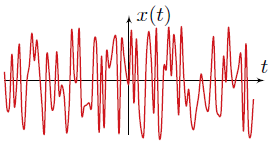
\includegraphics[width=0.4\columnwidth]{Images/stochastisch} \\ \midrule
	\textbf{Zeitkontinuerlich:} $x(t)$ ist definiert $t \in \mathbb{R}$
	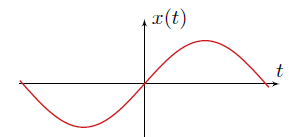
\includegraphics[width=0.4\columnwidth]{Images/Zeitkontinuerlich}
	& \textbf{Zeitdiskret:} $x(t)$ ist definiert bei $x(nT)$
	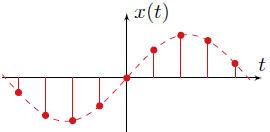
\includegraphics[width=0.4\columnwidth]{Images/zeitdiskret} \\ \midrule
	\textbf{Amplitudenkontinuierlich:} $x(t) = y$ mit $y \in  \mathbb{R}$	
	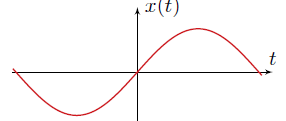
\includegraphics[width=0.4\columnwidth]{Images/Amplitudenkontinuierlich}
	& \textbf{Quantisiert:} $x(t) = y_k$ mit $y_k \in \mathbb{Z}$
	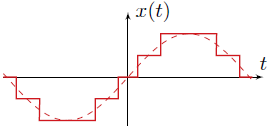
\includegraphics[width=0.4\columnwidth]{Images/quantisiert}\\ \midrule
	\textbf{Analog:} Zeit-undAmplitudenkontinuirlich
	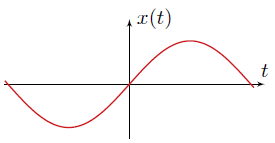
\includegraphics[width=0.4\columnwidth]{Images/analog}
	& \textbf{Digital:} Zeitdiskret und Quantisiert
	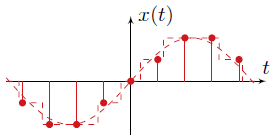
\includegraphics[width=0.4\columnwidth]{Images/digital}	
\end{tabular}

\subsection{Kenngrössen} 
\script{13} Kenngrössen beschreiben Signale und deren Eigenschaften.\\
\includegraphics[width=\columnwidth]{Images/kenngrössen}

\begin{tabular}{m{3cm} m{5cm}}
		Peak-To-Peak: & $x_{pp} = \max(x(t)) - \min(x(t))$ \\ \midrule
		Peak-Amplitude: & $x_p = \max(|x(t)|)$ \\\midrule
		Linear Mittelwert: & $\overline{x} = \langle x(t)\rangle = \lim\limits_{T\rightarrow\infty}\frac{1}{T}\int\limits_{-T/2}^{T/2}x(t)dt$ \\\midrule
		Momentanleistung: & $P_x(t) = |x(t)|^2$ \\\midrule
		Signalenergie: & $E_x = \int\limits_{-\infty}^{\infty}|x(t)|^2 dt \eqi \frac{1}{2\pi}\int\limits_{-\infty}^{\infty}|X(\omega)|^2d\omega$ \\\midrule
		Mittlere Leistung & $\overline{P}_x = \langle P_x(t)\rangle = \lim\limits_{T\rightarrow\infty}\frac{1}{T}\int\limits_{-T/2}^{T/2}|x(t)|^2dt \eqi \sum\limits_{n=-\infty}^{\infty}|c_n|^2$  \\\midrule
		Effektivwert: & $x_{eff} = x_{rms} = \sqrt{\overline{P}_x}$ \\\midrule
		Scheitelfaktor$^*$: & $C = \frac{x_p}{\sqrt{\overline{P}_x}}$
\end{tabular}
~\\ \\
$^*$: Der Scheitelfaktor: Grosses $C$ bedeutet, grosse Amplitude mit wenig Signalleistung, was schlecht ist.


\subsection{Leistungsverhältnisse}
\script{16}Um Leistungen mit zwei Signalen zu vergleichen werden überlicherweise logarithmische Skalen verwendet, um grosse Messbereiche abdecken zu können. Mit Dezibel werden Leistungspegel und keine Amplituden verglichen.

[B] (Bel) ist ein $\log_{10}$ einer Leistung.
\[k_{\text{P}} = 10 \cdot \log_{10}\left(\frac{P_y}{P_x}\right) \qquad [dB]\]

\textbf{ACHTUNG}: Bei Effektivwerten (RMS) wie Spannungspegel oder Strompegel wird mit $20$ multipliziert!
\[k_{\text{P dB}} = 20 \cdot \log_{10}\left(\frac{y_{rms}}{x_{rms}}\right) \qquad [dB]\]

\noindent\textbf{Dezibel-Verhätnisse}\\
\begin{table}[H]
	\begin{tabular}{r|c|c}
		& Leistungsverhätnis & Amplitudenverhätnis \\		\toprule
		$20dB$ & $100$ & $10$ \\ \midrule
		$10dB$ & $10$ & $\sqrt{10}$ \\\midrule
		$6dB$ & $4$ & $2$ \\\midrule
		$3dB$ & $2$ & $\sqrt{2}$ \\\midrule
		$0dB$ & $1$ & $1$ \\\midrule
		$-3dB$ & $\frac{1}{2}$ & $\frac{1}{\sqrt{2}}$ \\\midrule
		$-6dB$ & $\frac{1}{4}$ & $\frac{1}{2}$ \\\midrule
		$-10dB$ & $\frac{1}{10}$ & $\frac{1}{\sqrt{10}}$ \\\midrule
		$-20dB$ & $\frac{1}{100}$ & $\frac{1}{10}$ \\\midrule
	\end{tabular}
\end{table}
\noindent\textbf{Referenzpegel} \script{18}
\begin{table}[H]
	\begin{tabular}{rl || rl}
		$dBW$: & $0dBW = 1W$ & $dBm$: & $0dBm = 1mW$ \\ \midrule
		$dBV$: & $0dBV = \frac{(1V)^2}{R_{ref}}$& $db\mu V$: & $0dB\mu V = \frac{(1\mu V)^2}{R_{ref}}$ 
	\end{tabular}
\end{table}

\noindent Bei Spannungspegeln muss der Referenzwiderstand berücksichtigt werden.\\
\begin{itemize}[nosep]
	\item HF-Technik: $R_{ref} = 50 \Omega$
	\item Telefonie:  $R_{ref} = 600 \Omega$
\end{itemize}

~\\
\noindent\textbf{Beispiel:} Eine Verstärkung mit 27dB ergibt eine vervielfachung um 500!
\begin{align*}
	27dB &= 10db + 10db +10db - 3db \\
	&= 10 \cdot 10 \cdot 10 \cdot 10 / 2 \\
	&= 500
\end{align*}